\documentclass[a4paper]{article}

%\usepackage[cm]{fullpage}
\usepackage[T1]{fontenc}
\usepackage[english]{babel}
\usepackage{textcomp}
\usepackage{multirow}
\usepackage{float}
\usepackage{fancyhdr}
\usepackage{pdfpages}

\usepackage{hyperref}
\hypersetup{
	pdfauthor = {Christian Wemstad},
	pdftitle = {eh2730: Procurement Project Plan},
	pdfsubject = {EH2730},
	pdfkeywords = {Procurement, elicitation, analyzation, verification and validation},
	pdfcreator = {LaTeX with hyperref package},
	pdfproducer = {latex}
}

\usepackage{graphicx}
\usepackage{amsmath}

\title{Assignment II: Requirements Specifications for ACME Power Company}
\author{Henrik Sohlberg <\href{mailto:hsoh@kth.se}{hsoh@kth.se}> %
\and Christian Wemstad <\href{mailto:wemstad@kth.se}{wemstad@kth.se}> %
}

\fancyhf{}
\fancyhead[LE,RO]{\slshape \rightmark}
\fancyhead[LO,RE]{\slshape \leftmark}
\fancyfoot[C]{\thepage}

\begin{document}
\thispagestyle{empty}
\maketitle
\thispagestyle{empty}
\pagestyle{empty}
\newpage
\section*{Version table}
\label{sec:version_tabel}
\begin{table}[H]
	\centering
	\begin{tabular}{|l|l|l|l|}
		\hline
			\textit{Version} & \textit{Change log} & \textit{User} & \textit{Date}\\
		\hline
		     v. 1 & First version & Mr. Wemstad and Mr. Sohlberg & \today \\
		\hline
	\end{tabular}
\end{table}
\newpage       
\tableofcontents
\newpage
\pagestyle{fancy}
\setcounter{page}{1}
\section{Background}



\addcontentsline{toc}{section}{References}
\begin{thebibliography}{99}     
	
%\bibitem{gott2} \emph{Gottesdiener, Ellen. \textsl{"The Software Requirements Memmory Jogger" chapter 2}. GOAL/QPC, 2005}


\end{thebibliography}
\clearpage
\appendix
%\section{Stakeholder Elicitation Plan}
%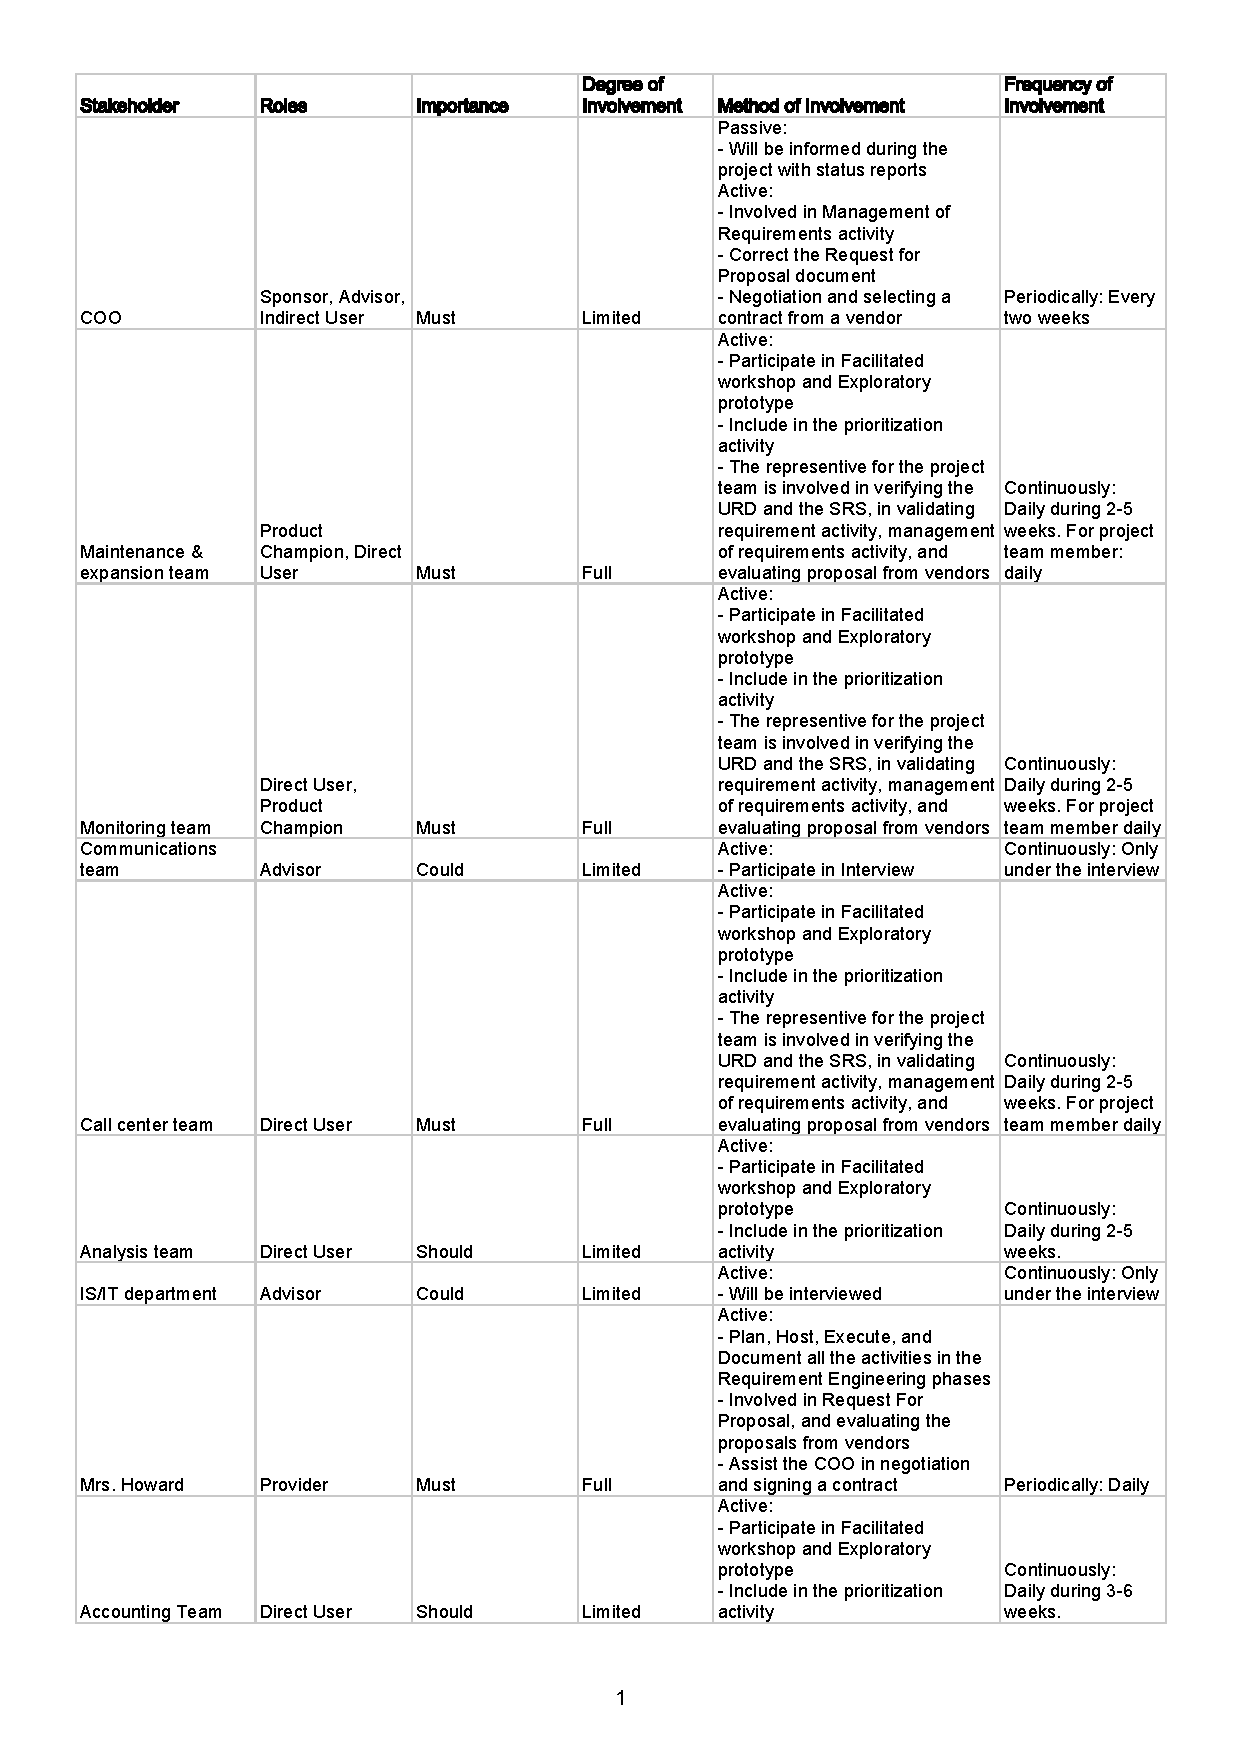
\includepdf[pages={-}]{appendix/stake_eli_plan.pdf}

\end{document}
